\begin{ejercicio}
    En un árbol \textbf{AVL} inicialmente vacío insertamos (por este orden) los siguientes elementos: \{8, 13, 10, 5, 11, 6, 7\}; y después eliminamos el 13. Mostrar la estructura del árbol antes y después de cada operación que requiera una rotación indicando de qué tipo es ésta.\\

    Las primeras inserciones no dan problemas, pero al insertar el 11 se produce un desequilibrio. En el nodo 13, el subárbol izquierdo tiene altura 2, mientras que el subárbol derecho tiene altura 0. Por tanto, hay que realizar una rotación hacia la derecha. Además, es doble, ya que el nodo desequilibrante (el 11) se encuentra en el subárbol derecho del subárbol izquierdo. El resultado de la rotación se ve en la Figura \ref{fig:AVL_Insertar11}.
    \begin{figure}[H]
        \centering
        \begin{subfigure}{0.45\textwidth}
            \centering
            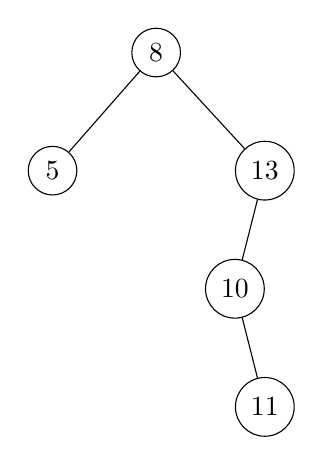
\begin{tikzpicture}[
                every node/.style={circle, draw},
                level 1/.style={sibling distance=2cm},
                level 2/.style={sibling distance=1cm},
                level 3/.style={sibling distance=1cm},
                level distance=1.5cm,
            ]
            \node {8}
            child[left] {node {5}}
            child[right] {node {13}
                child[left] {node {10}
                    child[right] {node {11}}
                }
            };
            \end{tikzpicture}
            \caption{\centering Estructura del AVL \ul{antes} de la rotación por el desequilibrio por del 11.}
        \end{subfigure}
        \hfill
        \begin{subfigure}{0.45\textwidth}
            \centering
            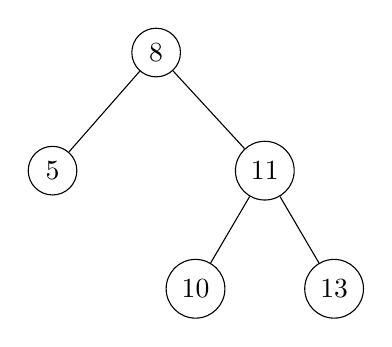
\begin{tikzpicture}[
                every node/.style={circle, draw},
                level 1/.style={sibling distance=2cm},
                level 2/.style={sibling distance=1cm},
                level 3/.style={sibling distance=1cm},
                level distance=1.5cm,
            ]
            \node {8}
            child[left] {node {5}}
            child[right] {node {11}
                child[left] {node {10}}
                child[right] {node {13}}
            };
            \end{tikzpicture}
            \caption{\centering Estructura del AVL \ul{después} de la rotación por el desequilibrio por del 11.}
        \end{subfigure}
        \caption{RDD en el nodo 13 por el desequilibrio que provoca la inserción del 11.}
        \label{fig:AVL_Insertar11}
    \end{figure}

    El insertado del 6 tampoco genera problemas, pero al insertar el 7, se desequilibria el 5. En este caso, se trata de una RSI, descrita en la Figura \ref{fig:AVL_Insertar7}.
    \begin{figure}[H]
        \centering
        \begin{subfigure}{0.45\textwidth}
            \centering
            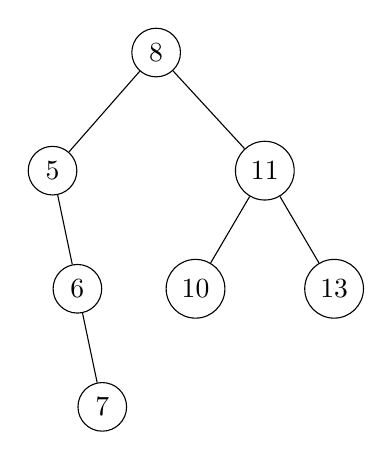
\begin{tikzpicture}[
                every node/.style={circle, draw},
                level 1/.style={sibling distance=2cm},
                level 2/.style={sibling distance=1cm},
                level 3/.style={sibling distance=1cm},
                level distance=1.5cm,
            ]
            \node {8}
            child[left] {node {5}
                child[right] {node {6}
                    child[right] {node {7}}
                }
            }
            child[right] {node {11}
                child[left] {node {10}}
                child[right] {node {13}}
            };
            \end{tikzpicture}
            \caption{\centering Estructura del AVL \ul{antes} de la rotación por el desequilibrio por del 7.}
        \end{subfigure}
        \hfill
        \begin{subfigure}{0.45\textwidth}
            \centering
            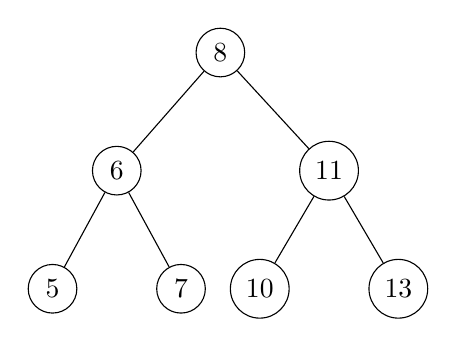
\begin{tikzpicture}[
                every node/.style={circle, draw},
                level 1/.style={sibling distance=2cm},
                level 2/.style={sibling distance=1cm},
                level 3/.style={sibling distance=1cm},
                level distance=1.5cm,
            ]
            \node {8}
            child[left] {node {6}
                child[left] {node {5}}
                child[right] {node {7}}
            }
            child[right] {node {11}
                child[left] {node {10}}
                child[right] {node {13}}
            };
            \end{tikzpicture}
            \caption{\centering Estructura del AVL \ul{después} de la rotación por el desequilibrio por del 7.}
        \end{subfigure}
        \caption{RSI en el nodo 5 por el desequilibrio que provoca la inserción del 7.}
        \label{fig:AVL_Insertar7}
    \end{figure}

    Respecto al borrado del nodo 13, el AVL queda como está representado en la Figura \ref{fig:AVL_Borrar13}. Vemos que ningún nodo queda desequilibrado, por lo que no son necesarias las rotaciones.
    \begin{figure}[H]
        \centering
        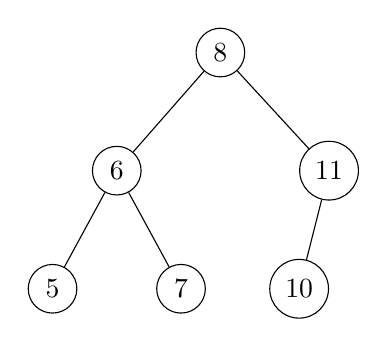
\begin{tikzpicture}[
            every node/.style={circle, draw},
            level 1/.style={sibling distance=2cm},
            level 2/.style={sibling distance=1cm},
            level 3/.style={sibling distance=1cm},
            level distance=1.5cm,
        ]
        \node {8}
        child[left] {node {6}
            child[left] {node {5}}
            child[right] {node {7}}
        }
        child[right] {node {11}
            child[left] {node {10}}
        };
        \end{tikzpicture}
        \caption{AVL tras el borrado del 13.}
        \label{fig:AVL_Borrar13}
    \end{figure}
\end{ejercicio}


\begin{ejercicio}
    Resuelva los siguientes ejercicios:
    \begin{enumerate}
        \item Insertar los enteros \{8,3,10,1,6,7,9,2,11\} en un \textbf{APO}. Obtener los árboles resultantes de aplicar el borrado dos veces.

        Tenemos que el APO tras insertar todos los elementos es el representado en la Figura \ref{fig:APO_Inicial}:
        \begin{figure}[H]
            \centering
            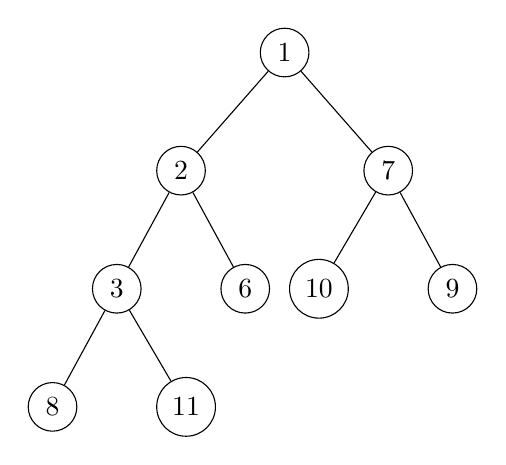
\begin{tikzpicture}[
                every node/.style={circle, draw},
                level 1/.style={sibling distance=2cm},
                level 2/.style={sibling distance=1cm},
                level 3/.style={sibling distance=1cm},
                level distance=1.5cm,
            ]
            \node {1}
            child[left] {node {2}
                child[left] {node {3}
                    child[left] {node {8}}
                    child[right] {node {11}}
                }
                child[right] {node {6}}
            }
            child[right] {node {7}
                child[left] {node {10}}
                child[right] {node {9}}
            };
            \end{tikzpicture}
            \caption{APO tras la inserción de todos los elementos.}
            \label{fig:APO_Inicial}
        \end{figure}


        Tras ejecutar el primer borrado, el APO queda representado en la Figura \ref{fig:APO_PrimerBorrado}, mientras que tras el segundo borrado se muestra en la Figura \ref{fig:APO_SegundorBorrado}:
        \begin{figure}[H]
            \centering
            \begin{subfigure}{0.45\textwidth}
                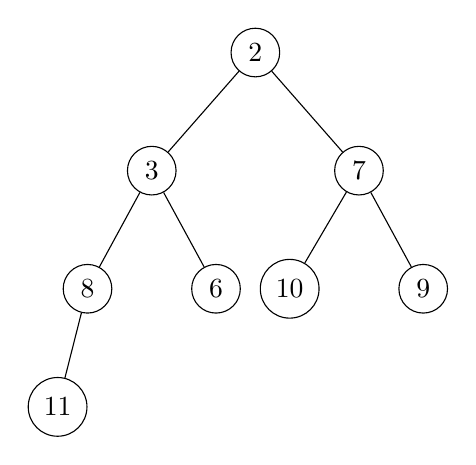
\begin{tikzpicture}[
                    every node/.style={circle, draw},
                    level 1/.style={sibling distance=2cm},
                    level 2/.style={sibling distance=1cm},
                    level 3/.style={sibling distance=1cm},
                    level distance=1.5cm,
                ]
                \node {2}
                child[left] {node {3}
                    child[left] {node {8}
                        child[left] {node {11}}
                    }
                    child[right] {node {6}}
                }
                child[right] {node {7}
                    child[left] {node {10}}
                    child[right] {node {9}}
                };
                \end{tikzpicture}
                \caption{APO tras el primer borrado.}
                \label{fig:APO_PrimerBorrado}
            \end{subfigure}
            \begin{subfigure}{0.45\textwidth}
                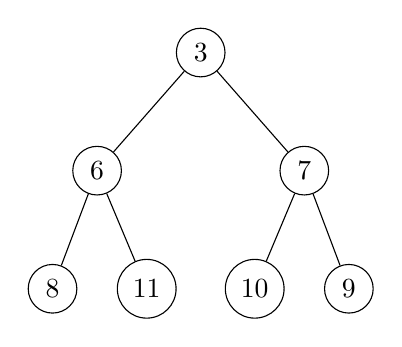
\begin{tikzpicture}[
                    every node/.style={circle, draw},
                    level 1/.style={sibling distance=2cm},
                    level 2/.style={sibling distance=0.5cm},
                    level 3/.style={sibling distance=0cm},
                    level distance=1.5cm,
                ]
                \node {3}
                child[left] {node {6}
                    child[left] {node {8}}
                    child[right] {node {11}}
                }
                child[right] {node {7}
                    child[left] {node {10}}
                    child[right] {node {9}}
                };
                \end{tikzpicture}
                \caption{APO tras el segundo borrado.}
                \label{fig:APO_SegundorBorrado}
            \end{subfigure}
            \caption{Dos borrados del APO de la Figura \ref{fig:APO_Inicial}.}
            \label{fig:APO_Borrados}
        \end{figure}
        \item Insertar las claves \{5, 13, 17, 38, 7, 59, 24, 62, 10, 11\} en una \textbf{Tabla Hash cerrada} de tamaño 11. A continuación borrar el 11 y el 38 y finalmente insertar el valor 49. Resolver las colisiones usando \textbf{hashing doble}.

        Como función hash, usamos $h(k)=k\% 11$. En el caso de que se produzcan colisiones, la función de rehashing que usamos es:
        \begin{equation*}
            h_i(k)=(h_{i-1}(k)+h_0(k))\% 11 \qquad \forall i=2,3,\dots \hspace{1cm} \left\{\begin{array}{l}
                h_0(k) =1+k\%9 \\
                h_1(k) = h(k)
            \end{array}\right.
        \end{equation*}

        Entonces, tenemos que:
        \begin{equation*}
            \begin{array}{rlll}
                h(5)&=5\\
                h(13)&=2\\
                h(17)&=6 \\
                h(38)&=5 &\qquad h_2(38)=5+h_0(38)=5+3=8\\
                h(7)&=7\\
                h(59)&=4\\
                h(24)&=2 &\qquad h_2(24)=2+h_0(24)=2+7=9\\
                h(62)&=7 &\qquad h_2(62)=(7+9)\%11=5 &\qquad h_3(62)=(5+9)\%11 = 3\\
                h(10)&=10\\
                h(11)&=0
            \end{array}
        \end{equation*}

        Tenemos que la tabla tras las primeras 10 inserciones queda conforme a la Tabla \ref{fig:TablaHashInicial}.
        \begin{table}
            \centering
            \begin{tabular}{c|c|c}
            Posición & Clave & Status \\ \hline \hline
            0        & 11       & O      \\
            1        &          & L      \\
            2        & 13       & O      \\
            3        & 62       & O      \\
            4        & 59       & O      \\
            5        & 5        & O      \\
            6        & 17       & O      \\
            7        & 7        & O      \\
            8        & 38       & O      \\
            9        & 24       & O      \\
            10       & 10       & O     
            \end{tabular}
            \caption{Tabla Hash cerrada tras las primeras 10 inserciones.}
            \label{fig:TablaHashInicial}
        \end{table}

        Tras el borrado del 11 y el 38, tan solo es necesario buscarlas y marcarlas como borradas. La tabla quedará como la Tabla \ref{fig:HashTrasBorrado}.
        \begin{table}
            \centering
            \begin{tabular}{c|c|c}
            Posición & Clave & Status \\ \hline \hline
            0        &          & B      \\
            1        &          & L      \\
            2        & 13       & O      \\
            3        & 62       & O      \\
            4        & 59       & O      \\
            5        & 5        & O      \\
            6        & 17       & O      \\
            7        & 7        & O      \\
            8        &          & B      \\
            9        & 24       & O      \\
            10       & 10       & O     
            \end{tabular}
            \caption{Tabla Hash cerrada tras el borrado del 11 y el 38.}
            \label{fig:HashTrasBorrado}
        \end{table}

        Insertamos ahora el 49. Veamos su posición:
        \begin{gather*}
            h(49)=5 \qquad h_2(49)=10 \qquad h_3(49)=(10+5)\%11=4
            \qquad h_4(49)=4+5=9 \\ h_5(49)=(9+5)\%11=3
            \qquad h_6(49)=3+5=8
        \end{gather*}

        Por tanto, insertamos el 49 en la posición 8, cuyo estado es B y por tanto, en términos de inseerción, disponemos de un hueco. La tabla quedará como la Tabla \ref{fig:HashTras49}.
        \begin{table}
            \centering
            \begin{tabular}{c|c|c}
            Posición & Clave & Status \\ \hline \hline
            0        &          & B      \\
            1        &          & L      \\
            2        & 13       & O      \\
            3        & 62       & O      \\
            4        & 59       & O      \\
            5        & 5        & O      \\
            6        & 17       & O      \\
            7        & 7        & O      \\
            8        & 49       & O      \\
            9        & 24       & O      \\
            10       & 10       & O     
            \end{tabular}
            \caption{Tabla Hash cerrada final tras la inserción del 49.}
            \label{fig:HashTras49}
        \end{table}
        
        
    \end{enumerate}
\end{ejercicio}